\documentclass[article]{jss}

\usepackage{orcidlink,thumbpdf,lmodern}
\usepackage{framed}
\newcommand{\class}[1]{`\code{#1}'}
\newcommand{\fct}[1]{\code{#1()}}

\usepackage{float}
\newfloat{listing}{htbp}{lop}
\floatname{listing}{Listing}



\author{Matthias Gondan~\orcidlink{0000-0001-9974-0057}\\Universit\"at Innsbruck
   \And Jan Wielemaker\\SWI-Prolog Solutions b.v.}
\Plainauthor{Matthias Gondan, Jan Wielemaker}

\title{\pkg{rolog}: \proglang{Prolog} queries from \proglang{R}}
\Plaintitle{rolog: Prolog queries from R}
\Shorttitle{\pkg{rolog}}

\Abstract{
  \proglang{Prolog} is a classical logic programming language with many
  applications in expert systems, computer linguistics and traditional, that is,
  symbolic artificial intelligence. The main strength of \proglang{Prolog} is
  its concise representation of facts and rules for the representation of
  knowledge and grammar, as well as its very efficient built-in search engine
  for closed world domains. \proglang{R} is a statistical programming language
  for data analysis and statistical modeling which is widely used in academia
  and industry. Besides the core library, a lot of packages have been developed
  for all kinds of statistical problems, including new-style artificial
  intelligence tools such as neural networks for machine learning and deep
  learning. Whereas \proglang{Prolog} is weak in statistical computation, but
  strong in symbolic manipulation, the converse may be said for 
  the \proglang{R} language. SWI-Prolog is a widely used \proglang{Prolog}
  system that offers a wide range of extensions for real world applications, and
  there already exist two \proglang{Prolog} ``packs'' to
  invoke \proglang{R} (\pkg{rserve-client}, \pkg{real}) from SWI-Prolog.
  However, given the large user community of \proglang{R}, there may also be a
  need for a connection in the reverse direction that allows 
  invoking \proglang{Prolog} queries in \proglang{R} computations. 
  The \proglang{R}\ package \pkg{rolog} embeds the SWI-Prolog system, thus
  enabling deterministic and non-deterministic queries to the Prolog
  interpreter. Usage of \pkg{rolog} is illustrated by a few examples.
}

\Keywords{Statistics; Logic Programming; Artificial Intelligence, \proglang{R}, \proglang{Prolog}}
\Plainkeywords{Statistics; Logic Programming; Artificial Intelligence, R, Prolog}

\Address{
  Matthias Gondan\\
  Department of Psychology\\
  University of Innsbruck\\
  Innrain 9\\
  A-6020 Innsbruck\\
  E-mail: \email{Matthias.Gondan-Rochon@uibk.ac.at}
}

\usepackage{Sweave}
\begin{document}
\Sconcordance{concordance:rolog.tex:rolog.Rnw:%
1 11 1 1 41 46 1 1 0 107 1 1 4 1 2 4 0 1 2 2 1 1 2 9 0 1 2 50 %
1 1 6 12 0 1 3 6 0 1 3 7 0 1 3 4 0 1 2 69 1 1 2 8 0 1 2 25 1 1 %
2 4 0 1 2 2 1 1 3 5 0 1 2 60 1 1 2 1 0 1 1 6 0 1 2 5 1 1 2 1 0 %
3 1 6 0 1 2 16 1 1 17 16 0 1 2 2 1 3 0 1 2 21 1 1 2 4 0 1 2 41 %
1 1 2 1 0 2 1 7 0 1 2 6 0 1 1 6 0 1 1 3 0 1 2 18 1 1 2 1 0 1 1 %
3 0 1 2 9 1 1 2 1 0 1 4 2 0 1 3 1 0 1 2 2 1 1 2 3 1 1 2 1 1 19 %
0 1 2 51 1 1 2 1 0 1 2 16 0 1 2 10 1 1 3 2 0 2 2 3 0 1 2 63 1 %
1 2 1 0 3 1 22 0 1 2 36 1 1 2 1 0 1 6 7 0 1 2 8 1 1 2 1 0 1 1 %
5 0 1 2 3 1 6 0 1 2 8 1 1 2 1 0 1 1 6 0 1 2 8 1 1 15 14 0 1 4 %
2 0 1 3 1 0 1 1 6 0 1 2 41 1 1 2 1 0 2 1 3 0 1 2 33 1 1 2 1 0 %
1 2 1 1 12 0 1 2 5 1 6 0 1 3 1 0 1 1 7 0 1 2 88 1}


\section[rolog: Prolog queries from R]{\pkg{rolog}: \proglang{Prolog} queries from \proglang{R}}
\label{sec:intro}

The \proglang{R} \citep{R} programming language and environment is a widely used
open source software for statistical data analysis. The basic \proglang{R} is a
functional language with lots of support for storage and manipulation of
different data types, and a strong emphasis on operations involving vectors and
arrays. Moreover, a huge number of
packages (e.g., CRAN, \url{https://cran.r-project.org/}) have been contributed
that cover problems from diverse areas such as bioinformatics, machine learning,
specialized statistical methods, web programming and connections to other
programming languages. An interface to \proglang{Prolog} is lacking so far.

The logic programming language \proglang{Prolog} was invented in the 1970ies 
by \citet{Colmerauer1996}, mostly for the purpose of natural language 
processing. Since then, logic programming has become an important driving force
in research on artificial intelligence, natural language processing, program
analysis, knowledge representation and theorem
proving \citep{Shoham1994,Lally2011,Carro2004,Hsiang1987}.  
SWI-Prolog \citep{Wielemaker2012} is an open-source implementation of Prolog
that mainly targets developers of applications, with many users in academia,
research and industry. SWI-Prolog includes a large number of libraries
for ``the real world'', for example, a web server, encryption, interfaces
to \proglang{C}/\proglang{C++} and other programming languages, as well as a
development environment and debugger. In addition, pluggable 
extensions (so-called packs) are available for specific tasks to enhance its
capabilities.

Unlike \proglang{R}, \proglang{Prolog} is a declarative programming language
consisting of facts and rules that define relations, for example, in a problem
space. \proglang{Prolog}'s major strength is its built-in query-driven search
engine that efficiently deals with complex structured data, with the data not
necessarily being numerical. In fact, \proglang{Prolog} only provides a basic
collection of arithmetic calculations via a purely functional
interface \code{is/2}. More complex calculations such as matrix
algebra, statistical models or machine learning need help from other systems,
for example, from \proglang{R}.

\citet{Angelopoulos2013} summarize work at the
intersection of symbolic knowledge representation and statistical inference,
especially in the area of model
fits \citep[EM algorithms, MCMC]{Sato2001,Angelopoulos2008} and stochastic logic
programs \citep{Cussens2000,Kimmig2011}. One of the major strengths of logic
programming is handling constraints; and a number of systems for constraint
satisfaction tools have been developed (constraint logic programming on
booleans, finite domains, reals, and intervals) for that
purpose \citep[e.g.,][]{Fruehwirth1998,Triska2018}. Some constraint handlers
exist in \proglang{R} (see the CRAN task view for optimization problems), but
more of them would be available via a bridge between \proglang{R}
and \proglang{Prolog}. 

Earlier approaches to connect \proglang{Prolog} and \proglang{R} have been
published as SWI-Prolog
packs \citep[real, rserve-client][]{Angelopoulos2013,Rserve} and as modules for
the YAP system \citep{YapR}. Whereas \pkg{real} establishes a direct link
to an embedded instance of \proglang{R}, \pkg{rserve-client} communicates with a
local or remote \proglang{R} service \citep{Urbanek2021}. The former approach
emphasizes speed, the latter might be preferred from a security perspective,
especially in systems such as SWISH \citep{SWISH} that accept only a set of
sandboxed commands for \proglang{Prolog}, but do not impose restrictions
on \proglang{R}. A common feature of the two packages is that they provide an
interface for \proglang{R} calls from \proglang{Prolog}, but not the other way
round, that is, querying \proglang{Prolog} from \proglang{R} is not possible, so
far.

\pkg{rolog} is an attempt to fill this gap, and to offer the possibility to raise
\proglang{Prolog} queries in \proglang{R} scripts, for example, to perform
efficient symbolic computations, searches in complex graphs, parsing natural
language and definite clause grammars. In addition, two \proglang{Prolog}
predicates are provided that enable \proglang{Prolog} to ring back to
the \proglang{R} system for bidirectional communication. Similar to \pkg{real}, 
tight communication between the two systems is established by linking to a
shared library that embeds the current version of SWI-Prolog. The exchange of
data is facilitated by the \proglang{C++} interfaces of the two
languages \citep{Edelbuettel2018,Wielemaker2021}. A less tight connection might
be established using the recently developed machine query
interface \citep[MQI]{Zinda2021} that allows socket-based communication between
foreign languages and SWI-Prolog (and, in fact, the \pkg{MQI} documentation
includes an example in which \proglang{R} is called).

A bidirectional bridge between \proglang{R} and \proglang{Prolog} might overcome
the limitations of both languages, thereby combining the extensive numerical and
statistical power of the \proglang{R} system with \proglang{Prolog}'s skills in
the representation of knowledge and reasoning. In addition to the useful little
tools shown in the examples below, \pkg{rolog} can therefore contribute to
progress at the intersection of traditional artificial intelligence and
contemporary statistical programming.

The next section presents the interface of \pkg{rolog} in detail. 
Section~\ref{sec:extending} presents possible extensions of the package at both
ends, in \proglang{R} and \proglang{Prolog}. Section~\ref{sec:examples} is a
list of illustrative examples that offer useful extensions to the \proglang{R}
system. Conclusions and further perspectives are summarized in 
Section~\ref{sec:conclusions}.

\section{Basic syntax}

\pkg{rolog} has a rather minimalistic syntax, providing only some basic
ingredients to establish communication with an embedded SWI-Prolog. The ways to
extend the interface are described in Section~\ref{sec:extending}.

After installation (in \proglang{R}, with \code{install.packages("rolog")}), the
package is loaded in the standard way
using \proglang{R}'s \code{library}-command.


\begin{Schunk}
\begin{Sinput}
R> library(rolog)
\end{Sinput}
\end{Schunk}

We can see SWI-Prolog's typical welcome message.

\begin{Schunk}
\begin{Soutput}
Welcome to SWI-Prolog (threaded, 64 bits, version 8.5.10-52-gcd28f88fd-DIRTY)
SWI-Prolog comes with ABSOLUTELY NO WARRANTY. This is free software.
Please run ?- license. for legal details.

For online help and background, visit https://www.swi-prolog.org
For built-in help, use ?- help(Topic). or ?- apropos(Word).
\end{Soutput}
\end{Schunk}

\subsection[R interface]{\proglang{R} interface}

Most of the work can done using the 
three \proglang{R}\ functions \code{query}, \code{submit}, and \code{clear}. The
functions \code{consult}, \code{once}, and \code{findall} are provided for
convenience.

\code{consult}. In most applications, a number of \proglang{Prolog} facts and
rules will be loaded into the system. To facilitate this recurrent task, 
the \proglang{Prolog} directive \code{consult/1} has been mirrored
into \proglang{R}, \code{consult(filename)}, with \emph{filename} given as a
string (or a list of strings if multiple files are to be consulted). Note that
the full filename should be given, including the extension (e.g., ``.pl'').
The function returns \code{TRUE} on success; in case of problems, it
returns \code{FALSE} and an error message is shown.

\code{query}. The function \code{query(call, options)} is used to create a
\proglang{Prolog} query (without invoking it yet). The first 
argument \emph{call} is a regular \proglang{R} call that is created 
using \proglang{R}'s function \code{call(name, ...)}. This call represents
the \proglang{Prolog} predicate which will be queried in the later course. The
creation of such predicates and \proglang{Prolog} terms is described below and
can become quite contrived (see the examples in Section\ 4). The second
argument, \emph{options}, may be used for ad hoc modifications of the
translation between \proglang{R} and \proglang{Prolog}, see the section below.
The function returns \code{TRUE} on success. Note that the function does not
check if the corresponding \proglang{Prolog} predicate actually exists (but 
see \code{submit()} below).

Only a single query can be opened at a given time. If a new query is created
while another query is still open, a warning is shown and the other query is
closed.

\code{submit}. Once a query has been created, it can be submitted
using \code{submit()}. If the query fails, the return value is \code{FALSE}. If
the query succeeds, a list of constraints is returned, with bindings for the
variables that satisfy the query. Repeated calls to submit are possible,
returning the different solutions of a query (until it eventually fails).
Programmatically distinguishing between the different types of return values for
success and failure (list vs. \code{FALSE}) is facilitated by 
the \proglang{R} function \code{isFALSE(x)}.

\code{clear}. Closes the query. The name of the function is chosen to avoid name
clashes with \proglang{R}'s own built-in function \code{close}. The function
returns an invisible \code{TRUE}, even if there is no open query.

The \proglang{R} program in Listing~\ref{listing1} illustrates a query 
to \proglang{Prolog}'s \code{member/2} using \pkg{rolog}'s syntax rules.

\begin{listing}[ht]
\begin{Schunk}
\begin{Sinput}
R> # member(1, [1, 2.0, a, "b", X])
R> # return value is TRUE (query successfully created), with an attribute
R> # that shows the prolog representation of the query
R> query(call("member", 
+             1L, list(1L, 2.0, quote(a), "b", expression(X), TRUE)))
\end{Sinput}
\begin{Soutput}
[1] TRUE
attr(,"query")
[1] "member(1, [1, 2.0, a, b, X, true])"
\end{Soutput}
\begin{Sinput}
R> # returns an empty list, stating that member(1, [1 | _]) is satisfied
R> submit()
\end{Sinput}
\begin{Soutput}
list()
\end{Soutput}
\begin{Sinput}
R> # returns a list, stating that the query is also satisfied if X = 1
R> submit()
\end{Sinput}
\begin{Soutput}
$X
[1] 1
\end{Soutput}
\begin{Sinput}
R> # close the query
R> clear()
\end{Sinput}
\end{Schunk}
\caption{A query to \proglang{Prolog}'s \code{member/2} predicate}
\label{listing1}
\end{listing}

\code{once} and \code{findall}. The function \code{once(call, options)} is a
convenience function that acts as a shortcut 
for \code{query(call, options)}, \code{submit()}, and \code{clear()}.
Similarly, \code{findall(call, options)} abbreviates the 
commands \code{query(call, options)}, repetition of \code{submit()} until
failure, and \code{clear()}, returning a list collecting the the return value of
the individual calls to submit.

\subsection[Creating Prolog terms in R]{Creating \proglang{Prolog} terms 
in \proglang{R}}

Table~\ref{tab1} summarizes the rules for the translation from \proglang{R} 
to \proglang{Prolog}. Most rules work in both directions, but a few exceptions
exist. For example, there is an empty atom in \proglang{Prolog}, but no empty
symbol in \proglang{R}, so the empty atom is translated to a character string
in \proglang{R}.

\begin{table}
\caption{Creating Prolog terms from R}
\label{tab1}
\begin{center}
\begin{tabular}{lll}
\hline
R                                      & Prolog                                       & Note/Alternatives              \\
\hline
\code{expression(X)}                   & Variable \code{X}                            & not necessarily uppercase in R \\
\code{as.symbol(abc)}                  & Atom \code{abc}                              & \code{as.name}, \code{quote}   \\
\code{TRUE}, \code{FALSE}, \code{NULL} & Atoms \code{true}, \code{false}, \code{null} &                                \\
\code{"abc"}                           & String \code{"abc"}                          &                                \\
\code{3L}                              & Integer \code{3}                             &                                \\
\code{3}                               & Float \code{3.0}                             &                                \\
\code{call("term", 1L, 2L)}            & Compound \code{term(1, 2)}                   & see below for \code{list()} and \code{c()} \\
\code{list(1L, 2L, 3L)}                & List \code{[1, 2, 3]}                        &                                \\
\code{list(a=1, b=2, c=3)}             & List \code{[a-1, b-2, c-3]}                  &                                \\
\code{c(1, 2, 3)}                      & \code{\#(1.0, 2.0, 3.0)}                     & vectors of length > 1          \\
\code{c(1L, 2L, 3L)} or \code{1:3}     & \code{\%(1, 2, 3)}                           &                                \\
\code{c("a", "b", "c")}                & \code{\$\$("a", "b", "c")}                   &                                \\
\code{c(TRUE, FALSE, NA)}              & \code{!(true, false, na)}                    &                                \\
\hline
\end{tabular}
\end{center}
\end{table}

Moreover, \proglang{R} is mostly vectorized, lacking support for scalar
entities (in \proglang{R}, scalar entities are treated as vectors of length\ 1.
Conversely, Prolog does not natively support vectors or matrices. The problem is
solved in the following way: 

\begin{itemize}
\item \proglang{R} vectors of length 0 are translated to \proglang{Prolog}'s
  empty list.
\item \proglang{R} vectors of length 1 are translated to \proglang{Prolog}
  scalars.
\item \proglang{R} vectors of length $N > 1$ are translated to \proglang{Prolog}
  terms \code{\#/N}, \code{\%/N}, \code{\$\$/N}, and \code{!/N} for floating
  point numbers, integers, strings and logicals, respectively.
\end{itemize}

In the reverse direction, \proglang{Prolog} terms like \code{\#/N} are
translated back to \proglang{R} vectors of length $N$, including 
terms \code{\#/0} and \code{\#/1} that map to \proglang{R} vectors of
length 0 and 1, respectively. To summarize, the rules for translation are not
fully symmetrical. A quick check for symmetry of the representation is obtained
by a query to \code{r_eval/2} (see also below, subsection \proglang{Prolog} 
interface):

\begin{Schunk}
\begin{Sinput}
R> once(call("r_eval", c(1, 2, NA, NaN, Inf), expression(X)))
\end{Sinput}
\begin{Soutput}
$X
[1]   1   2  NA NaN Inf
\end{Soutput}
\end{Schunk}

\subsection{Package options}

A few package-specific options have been defined to allow some fine-tuning of
the rules for translation between \proglang{R} and \proglang{Prolog}.

\begin{itemize}
\item \emph{realvec} (string): Name of the \proglang{Prolog} term for vectors of
  floats (default is \code{\#})
\item \emph{intvec} (string): same for vectors of integers (default is \code{\%})
\item \emph{boolvec} (string): same for vectors of logicals (default is \code{!})
\item \emph{charvec} (string): same for vectors of character strings (default
  is \code{\$\$}). The single dollar cannot be used because it is the list
  operator in \proglang{R}.
\item \emph{scalar} (logical): if \code{TRUE} (default), \proglang{R} vectors of
  length\ 1 are translated to scalars in Prolog. 
  If \code{FALSE}, \proglang{R}\ vectors are always translated to \code{\#/N}
  etc., depending on the type.
\item \emph{portray} (logical): if \code{TRUE} (default in \code{query}), the
  result of \code{query}, \code{once} and \code{findall} includes an attribute 
  with a representation of the query in \proglang{Prolog}.
\end{itemize}

The command \code{rolog_options()} returns a list with all the options. The 
options can be globally modified like this:

\begin{Schunk}
\begin{Sinput}
R> options(rolog.intvec="%%")
\end{Sinput}
\end{Schunk}

In a given query, the options can be set in the optional argument, for example,

\begin{Schunk}
\begin{Sinput}
R> query(call("member", expression(X), list(1:3, 4:6)),
+        options=list(intvec="%%"))
\end{Sinput}
\end{Schunk}

\subsection[Prolog interface]{\proglang{Prolog} interface}

\pkg{rolog} offers some basic support to call \proglang{R} 
from \proglang{Prolog}, that is, connecting the two systems in the reverse
direction. Two predicates can be used for this purpose, \code{r_eval(Call)}
and \code{r_eval(Function, Result)}. The former just invokes \proglang{R} with
the command \emph{Call} (ignoring the result); the latter 
evaluates \emph{Function} and unifies the result with \emph{Result}. Note that
proper quoting of \proglang{R} functions is needed at the \proglang{Prolog} end,
especially with \proglang{R} functions that start with uppercase letters or
contain a dot in their name.

Two use cases for \code{r_eval/2} are shown in Section\ 4 below.

\section{Extending the package}
\label{sec:extending}

The package is intentionally kept minimalistic, but can easily be extended by
convenience functions on both ends, \proglang{Prolog} and \proglang{R}, to
facilitate recurrent tasks and/or avoid cumbersome syntax. \proglang{R} is a
functional language, whereas \proglang{Prolog} is declarative. Obviously, there
cannot be a perfect one-to-one correspondence between the syntactic components
of two programming languages that follow completely different paradigms. Whereas
symbols, functions, numbers and character strings are easily mapped 
between \proglang{R} and \proglang{Prolog}, there are loose ends at both sides.
In particular, \proglang{Prolog} variables are translated from and 
to \proglang{R} \emph{expressions} (not to be confused with \proglang{R}
symbols), and \proglang{R} vectors of length $N > 1$ are translated to
the \proglang{Prolog} terms \code{\#/N}, \code{\%/N}, \code{!/N}, 
and \code{\$\$/N}, as mentioned above. These rules are, in principle, arbitrary
and can be intercepted at several stages. The process is illustrated 
in Figure~\ref{fig:workflow}. 

\begin{itemize}
\item \proglang{R} functions that may be used to pre-process 
  specific \proglang{R} elements before translation
  to \proglang{Prolog} (see, e.g., the \proglang{R} function \code{as.rolog()})
\item \proglang{Prolog} wrappers that manipulate the term before it is called
  and afterwards (see the example with dicts below)
\item \proglang{R} functions that post-process the result of a query
\end{itemize}

\begin{figure}[b]
\centering
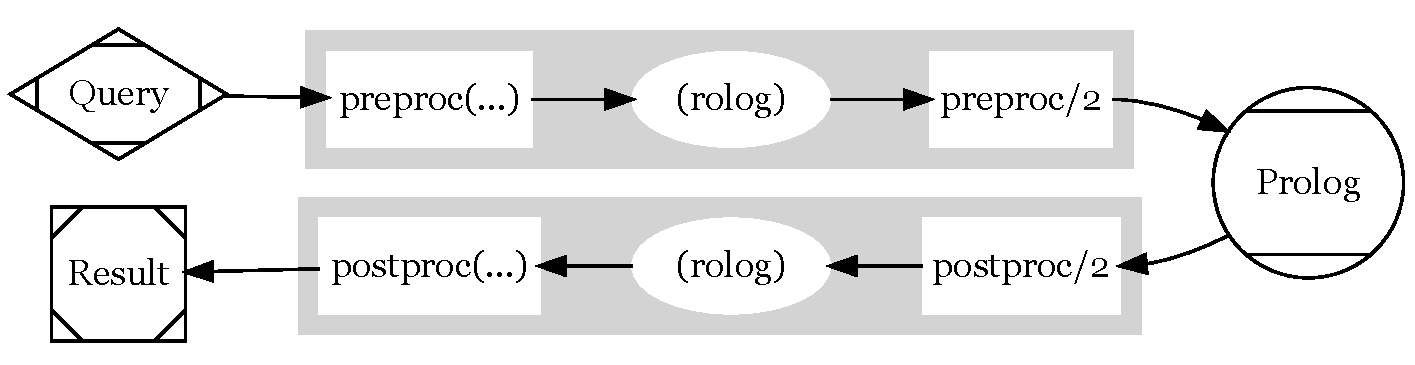
\includegraphics[width=0.8\columnwidth]{workflow}
\caption[Workflow in rolog]{Workflow in \pkg{rolog}}
\label{fig:workflow}
\end{figure}

\subsection[Pre-processing in R]{Pre-processing in \proglang{R}}

We have seen above that raising even simple everyday \proglang{Prolog} queries
such as \code{member(X, [1, 2, 3, a, b])} require 
complicated \proglang{R} expressions such as
\code{call("member", expression(X), list(1, 2, 3, quote(a), quote(b)))}.
The \proglang{R} function \code{as.rolog(Call)} is meant to simplify this a bit
by translating symbols starting with a dot to \proglang{Prolog} variables, and 
calls like \code{""[1, 2, 3, a, b]} to lists. The argument \emph{Call} is 
typically a quoted \proglang{R} call or symbol:

\begin{Schunk}
\begin{Sinput}
R> q <- quote(member(.X, ""[1, 2, 3, a, b]))
R> as.rolog(q)
\end{Sinput}
\begin{Soutput}
member(expression(X), list(1, 2, 3, a, b))
\end{Soutput}
\end{Schunk}

Note that the name of the variable will still be \emph{X} in the later course, 
not ``dot-X''. A bit flexibility is lost because \code{quote()} treats the
arguments \code{a}, \code{b} as symbols; to evaluate the respective 
variables (i.e., ``unquote''), they can be put in parentheses:

\begin{Schunk}
\begin{Sinput}
R> a <- 4
R> b <- 5
R> q <- quote(member(.X, ""[1, 2, 3, a, (b)]))
R> as.rolog(q)
\end{Sinput}
\begin{Soutput}
member(expression(X), list(1, 2, 3, a, 5))
\end{Soutput}
\end{Schunk}

Section~\ref{sec:examples} includes an example for mathematical rendering 
of \proglang{R} expressions. In that example, a pre-processing function is used
to bring function calls with named arguments to a canonical form which is then
handled in \proglang{Prolog}. More sophisticated work with quasi-quotations and
unquoting expressions is described in ``Advanced R'' \citep{Wickham2019}.

\subsection[Post-processing in R]{Post-processing in \proglang{R}}

This may again be a function that reverts some of the manipulations during
pre-processing. For \code{once()} and \code{submit()}, such a function would
operate on the bindings. For example, many \proglang{Prolog} programmers are
used to operate with atoms instead of character strings, whereas the latter is
the preferred representation of symbolic information in \proglang{R}. The
following simple example illustrates conversion of the results for a query
like \code{member(X, [a, b, c])} to strings.

\begin{Schunk}
\begin{Sinput}
R> stringify <- function(x)
+  {
+    # replace Prolog variable by the value of the R variable
+    if(is.name(x))
+      return(as.character(x))
+  
+    # Recurse into lists and calls
+    if(is.call(x))
+      x[-1] <- lapply(x[-1], FUN=stringify)
+  
+    if(is.list(x))
+      x <- lapply(x, FUN=stringify)
+  
+    # Leave the rest unchanged
+    return(x)
+  }
R> q <- quote(member(.X, ""[a, b, c]))
R> r <- findall(as.rolog(q))
R> stringify(r)
\end{Sinput}
\end{Schunk}

\subsection[Pre- and post-processing in Prolog]{Pre- and post-processing in \proglang{Prolog}}

Recent versions of SWI-Prolog support so-called dictionaries of the 
form \code{Tag{Key1:Value1, Key2:Value2, ...}}. The tag is typically an 
atom (but can be a variable, as well), the keys are unique atom or integers;
the values can be anything. Suppose we have a \proglang{Prolog} predicate that
does something with dicts, and we would like to query it from \proglang{R}. The
simplest solution is a wrapper in \proglang{Prolog} that 
translates \emph{key}-\emph{value} pairs \code{[Key1-Value1, Key2-Value2, ...]}
back and forth to dicts:

\begin{verbatim}
do_something_with_pairs(Pairs0, Pairs1) :-
    dict_pairs(Dict0, my_dict, Pairs0),
    do_something_with_dicts(Dict0, Dict1),
    dict_pairs(Dict1, my_dict, Pairs1).
\end{verbatim}

\code{do\_something\_with\_pairs/2} can then be queried from \proglang{R} using, 
for example, lists with named elements (see Table~\ref{tab1}).

\begin{Schunk}
\begin{Sinput}
R> once(call("do_something_with_pairs", list(a=1, b=2), expression(X)))
\end{Sinput}
\end{Schunk}

In the code above, \code{dict\_pairs/2} takes the role of both \code{preproc/2}
and \code{postproc/2} in Figure~\ref{fig:workflow}. It illustrates that
complicated syntax on the \proglang{R} side can be much simplified when doing
the conversion at the \proglang{Prolog} end. Ways to extend \proglang{Prolog} by
add-ons (``packs'') are shown in the next section.

\section{Examples}
\label{sec:examples}

In this section we present a few usage examples for the \pkg{rolog} package in
increasing complexity. Although the code snippets are mostly self-explanatory,
some familiarity with the \proglang{Prolog} language is helpful.

\subsection{Hello, world}

\proglang{Prolog}'s typical \emph{hello world} example is a search through a
directed acyclic graph (DAG), for example, a family tree like the one given in
Listing~\ref{lst:family}.

\begin{listing}
\begin{verbatim}
parent(pam, bob). parent(bob, ann). parent(bob, pat). parent(pat, jim).

ancestor(X, Z) :-
    parent(X, Z).

ancestor(X, Z) :-
    parent(X, Y),
    ancestor(Y, Z).
\end{verbatim}
\caption{A family tree in Prolog (see also \code{family.pl} in the 
  ``pl'' folder of the package)}
\label{lst:family}
\end{listing}

Listing~\ref{lst:family} is included in the package is accessed using the
function \code{system.file(...)}. Within \proglang{Prolog}, the normal workflow
is to consult the code with \code{[family]} and then to raise queries such
as \code{ancestor(X, jim)}, which returns, one by one, four solutions for the
variable \emph{X}. In \proglang{R}, we obtain the following results:

\begin{Schunk}
\begin{Sinput}
R> library(rolog)
R> consult(system.file(file.path("pl", "family.pl"), package="rolog"))
R> query(call("ancestor", expression(X), quote(jim)))
\end{Sinput}
\begin{Soutput}
[1] TRUE
attr(,"query")
[1] "ancestor(X, jim)"
\end{Soutput}
\begin{Sinput}
R> submit()        # solutions for X
\end{Sinput}
\begin{Soutput}
$X
pat
\end{Soutput}
\begin{Sinput}
R> submit()        # etc.
\end{Sinput}
\begin{Soutput}
$X
pam
\end{Soutput}
\begin{Sinput}
R> clear()         # close the query
\end{Sinput}
\end{Schunk}

As stated above, \code{consult()} loads the facts and rules of 
Listing~\ref{lst:family} into the \proglang{Prolog} 
database. \code{query(expr)} initializes the query \emph{expr}, and the
subsequent calls to \code{submit} return the conditions under which the query
succeeds. In this example, the query succeeds if \emph{X} is
either \code{pat}, \code{pam}, or \code{bob}. A query is closed
with \code{clear()}, or automatically if the query fails. Note that it is
generally not possible to open two queries simultaneously, so opening a
second query while another one is still open will raise a warning. If we are
interested in just the first solution, we can use \code{once(expr)} as a
shortcut to \code{query(expr)}, then \code{submit()}, then \code{clear()}. If we
want to collect all solutions of a query with a finite set of solutions, we can
use \code{findall(expr)}.

As mentioned in Section~\ref{sec:extending}, a simplified syntax is provided
by \code{as.rolog(...)} that accepts quoted expressions with dots 
indicating \proglang{Prolog} variables:

\begin{Schunk}
\begin{Sinput}
R> q <- quote(ancestor(.X, jim))
R> findall(as.rolog(q))
\end{Sinput}
\end{Schunk}

\subsection{Backdoor test}

A useful application of DAGs is confounder adjustment in causal 
analysis \citep{greenland1999,ggdag}. The \proglang{Prolog} 
file \code{backdoor.pl} is an implementation of Greenland et al.'s criteria for
the backdoor test for $d$-separation in DAGs, with a predicate \code{minimal/3}
that searches for minimally sufficient sets of variables for confounder
adjustment on the causal path between exposure and outcome.

\begin{Schunk}
\begin{Sinput}
R> consult(system.file(file.path("pl", "backdoor.pl"), package="rolog"))
R> # Figure 12 in Greenland et al.
R> add_node <- function(N)
+  	invisible(once(call("assert", call("node", N))))
R> add_arrow <- function(X, Y)
+  	invisible(once(call("assert", call("arrow", X, Y))))
R> add_node("a"); add_node("b"); add_node("c"); add_node("f"); add_node("u")
R> add_node("d") # outcome
R> add_node("e") # exposure
R> add_arrow("a", "d"); add_arrow("a", "f"); add_arrow("b", "d")
R> add_arrow("b", "f"); add_arrow("c", "d"); add_arrow("c", "f")
R> add_arrow("e", "d"); add_arrow("f", "e"); add_arrow("u", "a")
R> add_arrow("u", "b"); add_arrow("u", "c")
R> r <- findall(call("minimal", "e", "d", expression(S)))
R> unlist(r, recursive=FALSE)
\end{Sinput}
\begin{Soutput}
$S
$S[[1]]
[1] "a"

$S[[2]]
[1] "b"

$S[[3]]
[1] "c"


$S
$S[[1]]
[1] "f"
\end{Soutput}
\end{Schunk}

The query to \code{minimal/3} returns two minimally sufficient sets of
covariates for confounder adjustment (namely, \{a, b, c\} and \{f\}). 
The extra line with \code{unlist} only serves to tighten the output.

\begin{listing}[th]
\begin{verbatim}
:- use_module(library(dcg/basics)).
s(s(NP, VP)) --> np(NP, C), blank, vp(VP, C).
np(NP, C) --> pn(NP, C).
np(np(Det, N), C) --> det(Det, C), blank, n(N, C).
np(np(Det, N, PP), C) --> det(Det, C), blank, n(N, C), blank, pp(PP).
vp(vp(V, NP), C) --> v(V, C), blank, np(NP, _).
vp(vp(V, NP, PP), C) --> v(V, C), blank, np(NP, _), blank, pp(PP).
pp(pp(P, NP)) --> p(P), blank, np(NP, _).
det(det(a), sg) --> `a`.
det(det(the), _) --> `the`.
pn(pn(john), sg) --> `john`.
n(n(man), sg) --> `man`.
n(n(men), pl) --> `men`.
n(n(telescope), sg) --> `telescope`.
v(v(sees), sg) --> `sees`.
v(v(see), pl) --> `see`.
p(p(with)) --> `with`.

% Translate R string to code points and invoke phrase/2
sentence(Tree, Sentence) :-
    string_codes(Sentence, Codes),
    phrase(s(Tree), Codes).
\end{verbatim}
\caption{Simple grammar and lexicon. \code{sentence/2} pre-processes the \proglang{R} call}
\label{lst:dcg}
\end{listing}

\subsection{Definite clause grammars}

One of the main driving forces of \proglang{Prolog} development was natural
language processing \citep{Dahl1981}. Therefore, the next example is an
illustration of sentence parsing using so-called definite clause grammars. As
Listing~\ref{lst:dcg} shows, \pkg{rolog} can access modules from SWI's standard
library (e.g., \code{"dcg/basics.pl"} below).

As in the first example, we first consult a little \proglang{Prolog} program 
with a minimalistic grammar and lexicon (Listing~\ref{lst:dcg}), and then raise
a query asking for the syntactic structure of ``john sees a man with a 
telescope''. Closer inspection of the two results reveals the two possible
meanings, ``john sees a man \emph{who carries} a telescope'' versus ``john sees
a man \emph{through} a telescope''. More \proglang{Prolog} examples of natural
language processing are found in \citet{Blackburn2005}, 
including the resolution of anaphoric references and the extraction of semantic
meaning.

\begin{Schunk}
\begin{Sinput}
R> consult(system.file(file.path("pl", "telescope.pl"), package="rolog"))
R> findall(call("sentence", 
+               expression(Tree), "john sees a man with a telescope"))
\end{Sinput}
\begin{Soutput}
[[1]]
[[1]]$Tree
s(pn(john), vp(v(sees), np(det(a), n(man), pp(p(with), np(det(a), 
    n(telescope))))))


[[2]]
[[2]]$Tree
s(pn(john), vp(v(sees), np(det(a), n(man)), pp(p(with), np(det(a), 
    n(telescope)))))
\end{Soutput}
\end{Schunk}

\subsection[Add-ons for Prolog]{Add-ons for \proglang{Prolog}}

In description of the previous example, I noted in passing that \pkg{rolog} can
access the built-in libraries of SWI-Prolog (e.g., by calls
to \code{use_module/1,2}). It is also possible to extend the installation by
add-ons, including add-ons that require compilation, if the build
tools (essentially, RTools under Windows) are properly configured. This is
illustrated below by the demo add-on \pkg{environ} \citep{Environ} that collects
the current environment variables.

\begin{Schunk}
\begin{Sinput}
R> once(call("pack_install", 
+            quote(environ), list(call("interactive", FALSE))))
R> once(call("use_module", call("library", quote(environ))))
R> once(call("environ", expression(X)))
\end{Sinput}
\end{Schunk}

The query then unifies \emph{X} with a list with \code{Key=Value} terms. The
purpose if this example is obviously not to mimic the built-in
function \code{Sys.getenv()} from R, but to illustrate the installation and 
usage of \proglang{Prolog} extensions from within \proglang{R}.\footnote{In most
situations, the user would install the pack from within \proglang{Prolog} with
\code{pack\_install(environ).}}

\subsection{Term manipulation}

\proglang{Prolog} is homoiconic, that is, code is data. In this example, we make
use of \proglang{Prolog}'s ability to match expressions against given patterns
and modify these expressions according to a few 
predefined ``buggy rules'' \citep{Brown1978}, inspired by recurrent mistakes in
the statistics exams of the first author's students. Consider the $t$-statistic
for comparing an observed group average to a population mean:

\begin{equation}
T = \frac{\overline{X} - \mu}{s / \sqrt{N}}
\end{equation}

Some mistakes may occur in this calculation, for example, omission of the
implicit parentheses around the numerator and the denominator when typing the
numbers into a calculator, resulting 
in $\overline{X} - \frac{\mu}{s} \div \sqrt{N}$, or forgetting the square root
around $N$, or both. \proglang{Prolog} code for the two buggy rules is given in
Listing~\ref{lst:buggy}.

\begin{listing}[ht]
\begin{verbatim}
% Correct step from task to solution
expert(tratio(X, Mu, S, N), frac(X - Mu, S / sqrt(N))).

% Mistakes
buggy(frac(X - Mu, S / SQRTN), X - frac(Mu, S) / SQRTN).
buggy(sqrt(N), N).

% Apply expert and buggy rules
step(X, Y) :-
    expert(X, Y).

step(X, Y) :-
    buggy(X, Y).

% Enter expressions
step(X, Y) :-
    compound(X),
    mapargs(search, X, Y),
    dif(X, Y).

% Search through problem space
search(X, X).

search(X, Z) :-
    step(X, Y),
    search(Y, Z).
\end{verbatim}
\caption[Manipulating terms in Prolog]{Manipulating terms in \proglang{Prolog}}
\label{lst:buggy}
\end{listing}

The little e-learning system shown in Listing~\ref{lst:buggy} (\code{buggy.pl})
is invoked using the R script below.

\begin{Schunk}
\begin{Sinput}
R> consult(system.file(file.path("pl", "buggy.pl"), package="rolog"))
R> q <- quote(search(tratio(x, mu, s, n), .S))
R> s <- findall(as.rolog(q))
R> unlist(s)
\end{Sinput}
\begin{Soutput}
$S
tratio(x, mu, s, n)

$S
frac(x - mu, s/sqrt(n))

$S
x - frac(mu, s)/sqrt(n)

$S
x - frac(mu, s)/n

$S
frac(x - mu, s/n)

$S
x - frac(mu, s)/n
\end{Soutput}
\end{Schunk}

The fourth and the sixth result are combinations of the two buggy 
rules (parenthesis, then square root, and the other way round). Some additional
filters would be needed to eliminate trivial and redundant solutions 
\citep[see, e.g., the chapter on generate-and-test in][]{Sterling1994}.

It should be mentioned that \proglang{R} is homoiconic, too, and 
the \proglang{Prolog} code above can, in principle, be rewritten in \proglang{R}
using non-standard evaluation
techniques \citep{Wickham2019}. \proglang{Prolog}'s inbuilt pattern matching
algorithm simplifies things a lot, though. An important feature of such a term 
manipulation is that the evaluation of the term can be postponed; for example, 
there is no need to instantiate the variables \emph{X}, \emph{Mu}, \emph{s},
and \emph{N} with given values before raising a query. This is especially
helpful for variables that may represent larger sets of data in later steps.

\subsection{Rendering mathematical expressions}

The \proglang{R} extension of the markdown language \citep{Xie2020} enables
reproducible statistical reports with nice typesetting in HTML, Microsoft Word,
and Latex. However, so far, \proglang{R} expressions such 
as \code{pbinom(k, N, p)} are typeset as-is; prettier mathematical expressions
such as $P_\mathrm{Bi}(X \le k; N, p)$ require Latex commands 
like \code{P\_/mathrm\{Bi\}/left(X /le k; N, p/right)}, which are
cumbersome to type in and hard to read even for simple equations. Since
recently, manual pages include support for mathematical 
expressions \citep{Sarkar2022}, which already is a big improvement.

Below \proglang{Prolog}'s grammar rules are used for an \emph{automatic}
translation of \proglang{R} expressions to MathML. The result can then be used
for calculations or it can be rendered on a web page. A limited set of rules for
translation from R to MathML is found in \code{pl/mathml.pl} of 
package \pkg{rolog}. The relevant code snippets are shown in the listings below,
along with their output.

\begin{listing}

\begin{Schunk}
\begin{Sinput}
R> consult(system.file(file.path("pl", "mathml.pl"), package="rolog"))
R> mathml = function(term)
+  {
+    t = once(call("r2mathml", term, expression(X)))
+    cat(paste(t$X, collapse=""))
+  }
\end{Sinput}
\end{Schunk}

\caption[Using rolog to generate MathML from R expressions]{Using \pkg{rolog} to generate MathML from \proglang{R} expressions}
\label{lst:mathml1}
\end{listing}

The first example is easy. At the \proglang{Prolog} end, there is a handler 
for \code{pbinom/3} that translates the term into a pretty MathML syntax
like $P_\mathrm{Bi}(X \le k; N, \pi)$.

\begin{Schunk}
\begin{Sinput}
R> term = quote(pbinom(k, N, p))
R> mathml(term)     # pretty print
\end{Sinput}
\begin{Soutput}
<math><mrow><msub><mi>P</mi><mtext>Bi</mtext></msub><mo>&af;</mo><mrow><mo>(</mo><mrow><mrow><mi>X</mi><mo>&le;</mo><mi>k</mi></mrow><mo>;</mo><mrow><mi>N</mi><mo>,</mo><mi>p</mi></mrow></mrow><mo>)</mo></mrow></mrow></math> 
\end{Soutput}
\begin{Sinput}
R> k = 10
R> N = 22
R> p = 0.4
R> eval(term)       # determine result
\end{Sinput}
\begin{Soutput}
[1] 0.77195
\end{Soutput}
\end{Schunk}

The next example is interesting because \proglang{Prolog} needs find out the
name of the integration variable for \code{sin}. For that purpose, \pkg{rolog}
provides a predicate \code{r\_eval/2} that calls \proglang{R} 
from \proglang{Prolog} (i.e., the reverse direction, see also next example).
Here, the predicate is used for the \proglang{R} 
function \code{formalArgs(args(sin))}, which returns the name of the function
argument of \code{sin}, that is, \emph{x}.

\begin{Schunk}
\begin{Sinput}
R> term = quote(integrate(sin, 0L, 2L*pi))
R> mathml(term)
\end{Sinput}
\begin{Soutput}
<math><mrow><munderover><mo>&int;</mo><mn>0</mn><mrow><mn>2</mn><mo>&#x2062;</mo><mi>&pi;</mi></mrow></munderover><mrow><mi>sin</mi><mo>&af;</mo><mrow><mo>(</mo><mi>x</mi><mo>)</mo></mrow></mrow><mspace width="thinmathspace"></mspace><mi>d</mi><mi>x</mi></mrow></math> 
\end{Soutput}
\end{Schunk}

Note that the \proglang{Prolog} end, the handler for \code{integrate/3} is
quite rigid; it only accepts the three
arguments \emph{FUN}, \emph{lower}, \emph{upper} (in that particular order), and
without names, that is, 
something like \code{integrate(sin, lower=0L, upper=2L * pi)} would not print
the desired result. Moreover, \code{integrate} does not return a number, but a
structured object with several slots.

\begin{Schunk}
\begin{Sinput}
R> canonical <- function(term)
+  {
+    if(is.call(term))
+    {
+      f <- match.fun(term[[1]])
+      if(!is.primitive(f))
+        term <- match.call(f, term)
+      
+      # Recurse into arguments
+      term[-1] <- lapply(term[-1], canonical)
+    }
+  
+    return(term)
+  }
R> # A custom function
R> g <- function(u)
+    sin(u)
R> # Mixture of (partially) named and positional arguments in unusual order
R> term <- quote(2L * integrate(low=-Inf, up=Inf, g)$value)
R> mathml(canonical(term))
\end{Sinput}
\begin{Soutput}
<math><mrow><mn>2</mn><mo>&sdot;</mo><mrow><munderover><mo>&int;</mo><mrow><mo>-</mo><mi>&#x221E;</mi></mrow><mi>&#x221E;</mi></munderover><mrow><mi>g</mi><mo>&af;</mo><mrow><mo>(</mo><mi>u</mi><mo>)</mo></mrow></mrow><mspace width="thinmathspace"></mspace><mi>d</mi><mi>u</mi></mrow></mrow></math> 
\end{Soutput}
\end{Schunk}

Therefore, \code{pl/mathml.pl} includes two handlers. One handler accepts
canonicalized terms with named 
arguments, \code{integrate(f=Fn, lower=Lower, upper=Upper)}. The extra
function \code{canonical()} applies \code{match.call()} to 
non-primitive \proglang{R} calls, basically cleaning up the arguments and
bringing them into the correct order. The other handler accepts terms of the
form \code{\$(integrate(Fn, Lower, Upper), value)} that are needed to access
the numerical result of the integral.

\subsection[Calling Prolog from R]{Calling \proglang{Prolog} from \proglang{R}}

The basic workflow of the bridge from \proglang{R} to \proglang{Prolog} is
to (A)~translate an \proglang{R}~expression into a \proglang{Prolog}
term (i.e., a predicate), (B)~query the predicate, and then, (C)~translate 
the result (i.e., the bindings of the variables) back to \proglang{R}. The
reverse direction is straightforward, we start by translating 
a \proglang{Prolog}~term to an \proglang{R}~expression (i.e. Step~C), evaluate
the \proglang{R}~expression, and then translate the result back to
a \proglang{Prolog}~term (Step~A). \pkg{rolog} provides two predicates for this
purpose, \code{r_eval(Expr)} and \code{r_eval(Expr, Res)}. The
former is used to invoke an \proglang{R}~expression \emph{Expr} for its side
effects (e.g., initializing a random number generator); it does not return a
result. The latter is used to evaluate the \proglang{R}~expression \emph{Expr}
and return the result \emph{Res}. The code snippet in
Listing~\ref{lst:reval} (\code{r\_eval.pl}) illustrates this behavior.

\begin{listing}
\begin{verbatim}
r_seed(Seed) :-
    r_eval('set.seed'(Seed)).

r_norm(N, L) :-
    r_eval(rnorm(N), L).
\end{verbatim}

\caption[Calling R from Prolog using r\_eval/1 and r\_eval/2.]{Calling \proglang{R} from \proglang{Prolog} using \code{r\_eval/1}
  and \code{r\_eval/2}. The \proglang{R}~call \code{set.seed} is quoted because
  the dot is an operator in \proglang{Prolog}.}
\label{lst:reval}
\end{listing}

\begin{Schunk}
\begin{Sinput}
R> consult(system.file(file.path("pl", "r_eval.pl"), package="rolog"))
R> once(call("r_seed", 1234))
R> once(call("r_norm", 3L, expression(X)))
\end{Sinput}
\end{Schunk}

The example in Listing~\ref{lst:reval} is a bit trivial, basically illustrating
the syntax and the workflow. More serious applications of \code{r\_eval/1,2} are
illustrated in the example on mathematical expressions where \code{r\_eval/2} is
used to obtain the name of a function argument, as well as in the next example
on interval arithmetic, where \code{r\_eval/2} is used to evaluate monotonically
behaving \proglang{R} functions.

\subsection{Interval arithmetic}

Let $\langle\ell, u\rangle$ denote a number between $\ell$ and $u$, $\ell\le u$.
It is easily verified that the result of the
difference $\langle\ell_1, u_1\rangle - \langle\ell_2, u_2\rangle$ is somewhere
in the interval $\langle \ell_1 - u_2, u_1 - \ell_2\rangle$, and a number of
rules exist for basic arithmetic operations and (piecewise) monotonically
behaving functions \citep{Hickey2001}. For ratios, denominators with mixed sign
yield two possible intervals, for example,
$\langle 1, 2\rangle / \langle -3, 3\rangle = \langle -\infty, 3\rangle \cup \langle 3, \infty\rangle$,
as shown in Figure~4 in Hickey et al.'s article. The number of possible
candidates increases if more complicated functions are involved, as unions of
intervals themselves appear as arguments (e.g., if $I_1 \cup I_2$ is added
to $I_3 \cup I_4$, the result
is $I_1 + I_3 \cup I_1 + I_4 \cup I_2 + I_3 \cup I_2 + I_4$). The bottom line is
that calculations in interval arithmetic are non-deterministic in nature, and
the number of possible results is not foreseeable and cannot, in general, be
vectorized as is often done in \proglang{R}. Use cases for interval arithmetic
are the control of limitations of floating-point representations in computer
hardware, but intervals can also be used to represent the result of measurements
with limited precision, or truncated intermediate results of students doing hand
calculations. A few rules for basic interval arithmetic are found
in \code{pl/interval.pl}; and examples are shown below. Again, in the example
below, \proglang{Prolog} rings back to \proglang{R} via \code{r_eval/2} to
determine the result of \code{dbinom(X, Size, Prob, Log)}.

\begin{Schunk}
\begin{Sinput}
R> consult(system.file(file.path("pl", "interval.pl"), package="rolog"))
R> q <- quote(int(`...`(1, 2) / `...`(-3, 3), .Res))
R> findall(as.rolog(q))
\end{Sinput}
\begin{Soutput}
[[1]]
[[1]]$Res
...(-Inf, -0.333333333333333)


[[2]]
[[2]]$Res
...(0.333333333333333, Inf)
\end{Soutput}
\begin{Sinput}
R> D  <- quote(`...`(5.7, 5.8))
R> mu <- 4
R> s  <- quote(`...`(3.8, 3.9))
R> N  <- 24L
R> tratio <- call("/", call("-", D, mu), call("/", s, call("sqrt", N)))
R> once(call("int", tratio, expression(Res)))
\end{Sinput}
\begin{Soutput}
$Res
...(2.13545259627251, 2.32056923000512)
\end{Soutput}
\begin{Sinput}
R> # Binomial density
R> prob = quote(`...`(0.2, 0.3))
R> once(call("int", call("dbinom", 4L, 10L, prob, FALSE), expression(Res)))
\end{Sinput}
\begin{Soutput}
$Res
...(0.088080384, 0.200120949)
\end{Soutput}
\end{Schunk}

The slightly cumbersome syntax for entering an interval $\langle \ell, u\rangle$
is due to the fact that the ellipsis is a reserved symbol in \proglang{R} and
cannot be used as an infix operator. A powerful and comprehensive system for
constraint logic programming over intervals is available as a \proglang{Prolog}
pack \citep{Workman2021} and can easily be connected to \proglang{R} using, for
example, the present package.

\section{Conclusions}
\label{sec:conclusions}

\proglang{R} has become the primary language for statistical programming and
data science, but is currently lacking support for traditional, symbolic
artificial intelligence. There are already two add-ons for SWI-Prolog that allow
to run \proglang{R} calculations from Prolog \citep{Angelopoulos2013,Rserve},
but a connection in the other direction was missing, so far. \pkg{rolog} bridges
this gap by providing an interface to a SWI-Prolog distribution embedded into
an \proglang{R} package. The communication between the two systems is mainly in
the form of queries from \proglang{R} to \proglang{Prolog}, but two predicates
allow \proglang{Prolog} to ring back and evaluate terms in \proglang{R}. The
design of the package is minimalistic, providing three main 
functions \code{query(...)}, \code{submit()}, and \code{clear()}, and a very
limited set of convenience tools (\code{consult(...)}, \code{once(...)}, 
and \code{findall(...)}) to facilitate recurrent everyday actions. As both
systems are homoiconic in nature, it was easy to establish a one-to-one
correspondence between many the elements of the two languages. Most
exceptions (e.g., lack of \proglang{R} support for empty symbols) can be
avoided and/or circumvented by wrapper functions at both ends.

Simple ways to extend the package have been described in 
Section~\ref{sec:extending}; such extensions could, for example, 
include \proglang{R} objects and structures like those returned by \code{lm},
or S4 classes. In many use cases, this may be realized by transforming
the \proglang{R} object to a list with named elements, and rebuild the
object on the \proglang{Prolog} end on an as-needed basis. After a query, the
process is reversed. If speed is an issue, more of these steps can, in
principle, be moved into the package and implemented in \pkg{Rcpp}.

\pkg{rolog}, thus, opens up a wide of applications in logic programming for
statisticians and researchers at the intersection of symbolic and connectionist
artificial intelligence, where concise knowledge representation is combined with
statistical power. Moreover, \pkg{rolog} provides starting points for useful
small-scale solutions for everyday issues in data science (term transformations,
pretty mathematical output, interval arithmetic, see 
Section~\ref{sec:examples}).

At its present stage, a major limitation of \pkg{rolog} is its relatively slow
speed. For example, translation of \proglang{R} lists or vectors to the
respective elements of the \proglang{Prolog} language (also lists, \code{\#/N})
is done element-wise, in both directions. The translation is optimized by
using \pkg{Rcpp} \citep{Edelbuettel2018}, but there remains an upper bound in
the efficiency, because \proglang{Prolog} does not support vectors or
matrices. Since \proglang{Prolog}'s primary purpose is not vector or matrix
calculation, this limitation may not show up in real-world applications.
Another issue, maybe a bit annoying, is the rather cumbersome syntax of the
interface, with the need for quoted calls and \proglang{R} expressions being a
bit misused for representing \proglang{Prolog} variables. \pkg{rolog} was
deliberately chosen to be minimalistic and, so far, only depends on 
base \proglang{R}. A more concise representation might be obtained by tools from
the ``Tidyverse'' ecosystem, as described in Chapter\ 19 of 
Advanced R \citep{Wickham2019}. Finally, at this stage, \pkg{rolog} is unable to
deal with cyclic 
terms (e.g., \code{once(call("=", expression(A), call("f", expression(A))))}
raises an error message).

\pkg{rolog} is available for \proglang{R} Version 4.2 and later, and can easily
be installed using the usual \code{install.packages("rolog")}. The source code
of the package is found at \url{https://github.com/mgondan/rolog/}, including
installation instructions for Unix, Windows and macOS.

\section*{Acknowledgment}

Development of the package profited substantially from 
the \proglang{Prolog} packs \pkg{rserve\_client} \citep{Rserve} 
and \pkg{real} \citep{Angelopoulos2013}. The project was financially supported
by the European Commission (Erasmus+ project QHelp, 2019-1-EE01-KA203-051708).

\section*{Note}

The results in this paper were obtained 
using \proglang{R}~4.2.0 with 
the \pkg{rolog}~0.9.4 package. \proglang{R} itself
and all packages used are available from the 
Comprehensive \proglang{R} Archive Network (CRAN) 
at \url{https://CRAN.R-project.org/}.

\bibliography{bibliography}

\end{document}
